\pdfoutput=1
\documentclass[11pt,a4paper]{article}

%=============================================================================
% ENCODING AND FONTS
%=============================================================================
\usepackage[utf8]{inputenc}
\usepackage[T1]{fontenc}
\usepackage{newtxtext}
\usepackage{newtxmath}

%=============================================================================
% PAGE LAYOUT AND TYPOGRAPHY
%=============================================================================
\usepackage[a4paper, margin=1in]{geometry}
\usepackage{microtype}
\usepackage{setspace}
\onehalfspacing

%=============================================================================
% MATH
%=============================================================================
\usepackage{mathtools}
\usepackage{amssymb}

%=============================================================================
% GRAPHICS AND FIGURES
%=============================================================================
\usepackage{graphicx}
\usepackage[font=small,labelfont=bf,format=hang]{caption}
\usepackage{subcaption}

%=============================================================================
% TABLES
%=============================================================================
\usepackage{booktabs}
\usepackage{array}
\usepackage{multirow}
\usepackage{tabularx}

%=============================================================================
% LISTS
%=============================================================================
\usepackage{enumitem}
\setlist{nosep}

%=============================================================================
% COLORS
%=============================================================================
\usepackage{xcolor}
\definecolor{linkblue}{RGB}{0,51,153}

%=============================================================================
% TIKZ FOR FIGURES
%=============================================================================
\usepackage{tikz}
\usetikzlibrary{shapes.geometric, arrows.meta, positioning, fit, calc}

%=============================================================================
% CITATIONS
%=============================================================================
\usepackage[numbers,sort&compress]{natbib}

%=============================================================================
% HYPERLINKS
%=============================================================================
\usepackage{hyperref}
\hypersetup{
    colorlinks=true,
    linkcolor=linkblue,
    citecolor=linkblue,
    urlcolor=linkblue,
    pdftitle={From Symbolic Agents to LLM-Powered Autonomy: A Comprehensive Survey on the Evolution of AI Agents},
    pdfsubject={Artificial Intelligence},
    pdfkeywords={AI agents, large language models, autonomous agents, multi-agent systems, survey},
    bookmarks=true,
    bookmarksopen=true,
}

%=============================================================================
% SMART CROSS-REFERENCES
%=============================================================================
\usepackage{cleveref}
\crefname{equation}{Eq.}{Eqs.}
\crefname{figure}{Fig.}{Figs.}
\crefname{table}{Table}{Tables}
\crefname{section}{Sec.}{Secs.}
\crefname{algorithm}{Algorithm}{Algorithms}

%=============================================================================
% DOCUMENT METADATA
%=============================================================================
\title{\textbf{From Symbolic Agents to LLM-Powered Autonomy:\\ A Comprehensive Survey on the Evolution of AI Agents}}

\author{AI-Assisted Survey}

\date{April 2026}

%=============================================================================
% DOCUMENT
%=============================================================================
\begin{document}

\maketitle

% --- ABSTRACT ---
\begin{abstract}
\noindent
The development of autonomous agents has been a central pursuit of artificial intelligence for over six decades. This survey provides a comprehensive account of the evolution of AI agents, tracing their intellectual lineage from symbolic planning systems and the Belief-Desire-Intention (BDI) model of the 1990s, through reinforcement learning agents of the 2000s--2010s, to the current paradigm of large language model (LLM)-based agents. We present a structured analysis of the core capabilities that define modern agents---reasoning, planning, memory, and tool use---examining foundational techniques including chain-of-thought prompting, ReAct, Tree of Thoughts, and Reflexion. We survey the major agent frameworks that have emerged since 2023, from early autonomous projects such as AutoGPT and BabyAGI to production-grade systems including LangChain, AutoGen, and CrewAI. We further examine the resurgence of multi-agent systems, where LLM-powered agents collaborate through natural language to tackle complex tasks in software development, scientific research, and web automation. Finally, we identify key open challenges---including reliability, safety, evaluation, and efficiency---and outline promising future directions such as learning from experience, multimodal agency, and human-agent collaboration. By connecting historical foundations with cutting-edge developments, this survey offers both newcomers and experienced researchers a unified perspective on where the field has been, where it stands, and where it is headed.

\vspace{0.5em}
\noindent
\textbf{Keywords:} AI agents, large language models, autonomous agents, multi-agent systems, tool use, planning, memory
\end{abstract}

% --- 1. INTRODUCTION ---
\section{Introduction}
\label{sec:intro}

The concept of an autonomous agent---an entity capable of perceiving its environment, reasoning about goals, and taking actions to achieve them---has been a central aspiration of artificial intelligence since its inception. From the early rule-based expert systems of the 1970s to the reinforcement learning breakthroughs of the 2010s, the pursuit of intelligent agency has driven some of the most significant advances in the field. However, the emergence of large language models (LLMs) such as GPT-3~\citep{brown2020language} and its instruction-tuned successors~\citep{ouyang2022training} has fundamentally transformed the landscape of agent research, enabling a new generation of systems that can understand natural language instructions, reason about complex tasks, and interact with diverse tools and environments.

The rapid proliferation of LLM-based agents since 2023 has been remarkable. Projects such as AutoGPT~\citep{autogpt2023} and BabyAGI~\citep{babyagi2023} captured widespread attention by demonstrating that LLMs could be orchestrated to autonomously decompose goals, execute multi-step plans, and self-correct based on feedback. Concurrently, academic research has produced foundational frameworks for agent reasoning, including ReAct~\citep{yao2023react}, Reflexion~\citep{shinn2024reflexion}, and Tree of Thoughts~\citep{yao2024tree}, which formalize how language models can synergize reasoning with action-taking. These developments have catalyzed an explosion of research spanning single-agent architectures, multi-agent collaboration, tool use, memory systems, and real-world applications.

Despite this rapid progress, the field lacks a unified narrative that traces the evolution of AI agents from their symbolic roots to the current LLM-powered paradigm. Existing surveys have provided valuable snapshots of specific aspects: Wang et al.~\citep{wang2024survey} offered a comprehensive taxonomy of LLM-based autonomous agents, Xi et al.~\citep{xi2023rise} examined the rise and potential of such systems, and Luo et al.~\citep{luo2025methodology} presented a methodology-centered analysis. However, few works have attempted to connect the historical foundations of agent research with the modern LLM-driven revolution in a single, coherent account.

This survey aims to fill that gap by providing a comprehensive overview of the evolution of AI agents, organized along both historical and thematic dimensions. Our contributions are as follows:

\begin{itemize}
    \item We trace the intellectual lineage of AI agents from symbolic AI and the Belief-Desire-Intention (BDI) model through reinforcement learning to the current LLM-based paradigm.
    \item We provide a structured analysis of the core capabilities that define modern LLM-based agents: reasoning, planning, memory, and tool use.
    \item We survey the major agent frameworks and multi-agent systems that have emerged since 2023, analyzing their architectural choices and trade-offs.
    \item We identify key applications, open challenges, and promising future directions for the field.
\end{itemize}

The remainder of this paper is organized as follows. \Cref{sec:background} establishes foundational definitions and a conceptual framework for understanding agents. \Cref{sec:early} reviews the pre-LLM history of agent research. \Cref{sec:llm-agents} examines the core techniques underlying LLM-based agents. \Cref{sec:frameworks} surveys major agent frameworks and toolkits. \Cref{sec:multiagent} discusses multi-agent systems. \Cref{sec:applications} presents applications and case studies. \Cref{sec:challenges} identifies challenges and future directions, and \Cref{sec:conclusion} concludes.

% --- 2. BACKGROUND AND DEFINITIONS ---
\section{Background and Definitions}
\label{sec:background}

\subsection{What Is an Agent?}

The term ``agent'' has been used with varying definitions across different communities. In the classical AI literature, Wooldridge and Jennings~\citep{wooldridge1995intelligent} defined an agent as a computer system situated in some environment that is capable of autonomous action in order to meet its design objectives. Russell and Norvig further refined this by characterizing an agent as anything that can be viewed as perceiving its environment through sensors and acting upon that environment through actuators.

In the context of LLM-based systems, we adopt a working definition that synthesizes these perspectives: an \textbf{AI agent} is a system that uses a language model as its core reasoning engine, augmented with the ability to perceive its environment, maintain internal state, make plans, and take actions---including the use of external tools---to accomplish goals specified in natural language.

\subsection{Core Components of Modern Agents}

Following the taxonomies proposed by Wang et al.~\citep{wang2024survey} and Xi et al.~\citep{xi2023rise}, we identify four core components that characterize modern LLM-based agents:

\begin{enumerate}
    \item \textbf{Perception}: The ability to receive and interpret inputs from the environment, including text, images, code, and structured data.
    \item \textbf{Reasoning and Planning}: The capacity to decompose complex goals into sub-tasks, evaluate alternative strategies, and construct executable plans. This encompasses techniques such as chain-of-thought prompting~\citep{wei2022chain}, tree search~\citep{yao2024tree}, and self-reflection~\citep{shinn2024reflexion}.
    \item \textbf{Memory}: Mechanisms for storing and retrieving information across interactions, including short-term working memory (conversation context), long-term episodic memory (past experiences), and semantic memory (factual knowledge).
    \item \textbf{Action and Tool Use}: The ability to execute actions in the environment, including calling APIs, running code, browsing the web, and manipulating files. Toolformer~\citep{schick2024toolformer} and ToolLLM~\citep{qin2023toolllm} demonstrated that LLMs can learn to use tools effectively.
\end{enumerate}

\begin{figure}[tbp]
\centering
\begin{tikzpicture}[
    node distance=0.8cm and 1.2cm,
    block/.style={rectangle, draw, rounded corners, minimum width=2.2cm, minimum height=0.8cm, align=center, font=\small},
    core/.style={block, fill=tolblue!20, draw=tolblue, thick},
    comp/.style={block, fill=tolorange!20, draw=tolorange},
    env/.style={block, fill=tolgreen!20, draw=tolgreen},
    arr/.style={-{Stealth[length=2.5mm]}, thick}
]
% Core LLM
\node[core, minimum width=3.5cm, minimum height=1.2cm] (llm) {\textbf{LLM Core}\\(Reasoning Engine)};

% Four components around the core
\node[comp, above=of llm] (plan) {Planning};
\node[comp, left=of llm] (mem) {Memory};
\node[comp, right=of llm] (tool) {Tool Use};
\node[comp, below=of llm] (percep) {Perception};

% Environment
\node[env, below=1.2cm of percep] (envnode) {Environment};

% Arrows
\draw[arr] (llm) -- (plan);
\draw[arr] (plan) -- (llm);
\draw[arr] (llm) -- (mem);
\draw[arr] (mem) -- (llm);
\draw[arr] (llm) -- (tool);
\draw[arr] (tool) -- (llm);
\draw[arr] (percep) -- (llm);
\draw[arr] (envnode) -- (percep);
\draw[arr] (tool) |- (envnode);

% Labels
\node[font=\tiny, right=0.1cm of plan.east, anchor=west, text=gray] {CoT, ReAct, ToT};
\node[font=\tiny, left=0.1cm of mem.west, anchor=east, text=gray] {Short/Long-term};
\node[font=\tiny, right=0.1cm of tool.east, anchor=west, text=gray] {APIs, Code, Web};
\end{tikzpicture}
\caption{Architecture of a typical LLM-based agent. The LLM serves as the central reasoning engine, interacting with four core modules: planning (task decomposition and strategy), memory (experience storage and retrieval), tool use (external API and environment interaction), and perception (input processing).}
\label{fig:agent-arch}
\end{figure}

\subsection{Taxonomy of Agent Architectures}

Agent architectures can be broadly classified along several dimensions:

\begin{itemize}
    \item \textbf{Single-agent vs. Multi-agent}: Whether the system consists of one agent or multiple collaborating agents.
    \item \textbf{Reactive vs. Deliberative}: Whether the agent responds directly to stimuli or engages in explicit planning and reasoning.
    \item \textbf{Monolithic vs. Modular}: Whether capabilities are integrated into a single model or distributed across specialized components.
    \item \textbf{Static vs. Adaptive}: Whether the agent's behavior is fixed or evolves through learning and self-improvement.
\end{itemize}

% --- 3. EARLY FOUNDATIONS ---
\section{Early Foundations of AI Agents}
\label{sec:early}

\subsection{Symbolic AI and Expert Systems (1960s--1990s)}

The earliest conceptions of artificial agents emerged from the symbolic AI tradition. Systems like STRIPS (Stanford Research Institute Problem Solver, 1971) introduced formal planning as a core agent capability, representing the world as a set of logical predicates and searching for action sequences that transform an initial state into a goal state. The General Problem Solver (GPS) by Newell and Simon (1963) embodied the idea that intelligence could be achieved through symbol manipulation and means-ends analysis.

Expert systems of the 1980s, such as MYCIN and DENDRAL, demonstrated that domain-specific knowledge could be encoded as production rules to create systems capable of reasoning and decision-making within narrow domains. While these systems lacked the generality and adaptability of modern agents, they established fundamental principles: the separation of knowledge from inference, the importance of explanation capabilities, and the value of modular knowledge representation.

\subsection{The BDI Model and Multi-Agent Systems (1990s)}

The Belief-Desire-Intention (BDI) model, formalized by Rao and Georgeff~\citep{rao1995bdi}, provided a philosophical and computational framework for rational agency. In this model, agents maintain beliefs about the world, desires representing their goals, and intentions that commit them to particular courses of action. The BDI architecture influenced a generation of agent platforms, including JACK, Jason, and Jadex, and remains relevant as a conceptual foundation for understanding modern agent behavior.

Concurrently, the multi-agent systems (MAS) community developed frameworks for agent communication, coordination, and negotiation. Standards such as FIPA-ACL (Foundation for Intelligent Physical Agents -- Agent Communication Language) established protocols for inter-agent messaging, while research on mechanism design and game theory provided formal tools for analyzing strategic interactions among self-interested agents.

Wooldridge and Jennings~\citep{wooldridge1995intelligent} provided an influential synthesis of agent theory and practice, identifying key properties of intelligent agents: autonomy, social ability, reactivity, and pro-activeness. These properties continue to serve as design criteria for modern agent systems.

\subsection{Reinforcement Learning Agents (2000s--2010s)}

The reinforcement learning (RL) paradigm, comprehensively described by Sutton and Barto~\citep{sutton2018reinforcement}, offered a fundamentally different approach to agent design. Rather than encoding knowledge explicitly, RL agents learn optimal behavior through trial-and-error interaction with their environment, guided by reward signals.

Key milestones in RL-based agency include: Deep Q-Networks (DQN)~\citep{mnih2015human} achieving human-level performance on Atari games; AlphaGo~\citep{silver2016mastering} defeating the world champion in Go through a combination of deep learning and Monte Carlo tree search; and OpenAI Five (2019) demonstrating coordinated multi-agent play in the complex real-time strategy game Dota 2.

While RL agents achieved remarkable performance in specific domains, they faced significant limitations: sample inefficiency requiring millions of interactions, difficulty in transferring learned policies across tasks, and the challenge of specifying reward functions for open-ended real-world tasks. These limitations set the stage for the LLM-based agent paradigm, which leverages the broad world knowledge and language understanding of pre-trained models to overcome many of these challenges.

\begin{figure}[tbp]
\centering
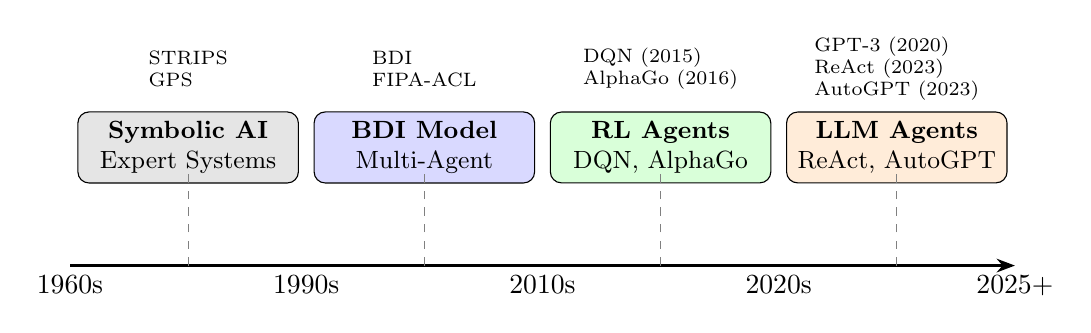
\begin{tikzpicture}[
    node distance=0.3cm,
    era/.style={rectangle, draw, rounded corners, minimum width=2.8cm, minimum height=0.7cm, align=center, font=\small},
    milestone/.style={font=\scriptsize, align=left}
]
% Timeline axis
\draw[thick, -Stealth] (0,0) -- (12,0);
\foreach \x/\year in {0/1960s, 3/1990s, 6/2010s, 9/2020s, 12/2025+}
    \node[below] at (\x,0) {\year};

% Era blocks
\node[era, fill=gray!20] at (1.5,1.5) {\textbf{Symbolic AI}\\Expert Systems};
\node[era, fill=blue!15] at (4.5,1.5) {\textbf{BDI Model}\\Multi-Agent};
\node[era, fill=green!15] at (7.5,1.5) {\textbf{RL Agents}\\DQN, AlphaGo};
\node[era, fill=orange!15] at (10.5,1.5) {\textbf{LLM Agents}\\ReAct, AutoGPT};

% Key milestones
\node[milestone] at (1.5,2.5) {STRIPS\\GPS};
\node[milestone] at (4.5,2.5) {BDI\\FIPA-ACL};
\node[milestone] at (7.5,2.5) {DQN (2015)\\AlphaGo (2016)};
\node[milestone] at (10.5,2.5) {GPT-3 (2020)\\ReAct (2023)\\AutoGPT (2023)};

% Connecting lines
\draw[dashed, gray] (1.5,0) -- (1.5,1.2);
\draw[dashed, gray] (4.5,0) -- (4.5,1.2);
\draw[dashed, gray] (7.5,0) -- (7.5,1.2);
\draw[dashed, gray] (10.5,0) -- (10.5,1.2);
\end{tikzpicture}
\caption{Timeline of AI agent evolution from symbolic systems (1960s--1990s) through BDI and multi-agent systems (1990s), reinforcement learning agents (2010s), to the current LLM-based paradigm (2020s--present).}
\label{fig:timeline}
\end{figure}

% --- 4. LLM-BASED AGENTS ---
\section{LLM-Based Agents}
\label{sec:llm-agents}

The emergence of large language models with strong instruction-following and reasoning capabilities has enabled a fundamentally new approach to building autonomous agents. Rather than learning from scratch through environment interaction, LLM-based agents leverage the vast knowledge encoded during pre-training to reason about tasks, generate plans, and interact with tools---all through natural language.

\subsection{Reasoning and Prompting Strategies}

The foundation of LLM-based agency lies in structured prompting strategies that elicit systematic reasoning from language models.

\paragraph{Chain-of-Thought (CoT).} Wei et al.~\citep{wei2022chain} demonstrated that prompting LLMs to generate intermediate reasoning steps dramatically improves performance on complex tasks. By including examples of step-by-step reasoning in the prompt, models learn to decompose problems and reason through them sequentially. This simple yet powerful technique laid the groundwork for more sophisticated agent reasoning.

\paragraph{ReAct.} Yao et al.~\citep{yao2023react} introduced the ReAct framework, which interleaves reasoning traces with action execution. In ReAct, the agent alternates between generating thoughts (reasoning about what to do next) and taking actions (such as searching the web or querying a database), using the observations from actions to inform subsequent reasoning. This tight coupling of reasoning and acting proved highly effective for tasks requiring interaction with external environments.

\paragraph{Tree of Thoughts (ToT).} Yao et al.~\citep{yao2024tree} extended chain-of-thought reasoning into a tree-structured search process. Rather than following a single reasoning chain, ToT explores multiple reasoning paths simultaneously, evaluates intermediate states, and backtracks when necessary. This deliberate problem-solving approach enables LLMs to tackle tasks that require exploration and strategic planning.

\paragraph{Self-Consistency.} Wang et al.~\citep{wang2024selfconsistency} proposed self-consistency decoding, which samples multiple reasoning paths and selects the most consistent answer through majority voting. This approach improves robustness over single-chain reasoning and has become a standard technique in agent systems that require reliable decision-making.

\paragraph{Reflexion.} Shinn et al.~\citep{shinn2024reflexion} proposed a framework for verbal reinforcement learning, where agents reflect on their failures and generate natural language feedback to improve future attempts. Unlike traditional RL, which requires scalar reward signals, Reflexion leverages the language model's ability to articulate what went wrong and how to improve, creating a self-improvement loop without parameter updates.

Sumers et al.~\citep{sumers2024cognitive} provided a unifying perspective on these techniques through the lens of cognitive architectures, proposing a framework that maps LLM agent designs to established cognitive science concepts including perception, memory, decision-making, and metacognition.

\subsection{Memory Systems}

Effective agency requires the ability to store and retrieve information across interactions. Park et al.~\citep{park2023generative} demonstrated the power of memory in their Generative Agents work, where simulated agents maintained detailed memories of their experiences, reflected on them to form higher-level abstractions, and used these memories to guide future behavior. Their architecture included three key components:

\begin{itemize}
    \item \textbf{Memory stream}: A comprehensive record of the agent's experiences, stored as natural language descriptions with timestamps.
    \item \textbf{Retrieval}: A mechanism that surfaces relevant memories based on recency, importance, and relevance to the current context.
    \item \textbf{Reflection}: A process that periodically synthesizes recent memories into higher-level insights and generalizations.
\end{itemize}

This memory architecture has influenced numerous subsequent systems and remains a reference design for agent memory.

\subsection{Tool Use and Environment Interaction}

A defining characteristic of LLM-based agents is their ability to use external tools to extend their capabilities beyond pure text generation.

Schick et al.~\citep{schick2024toolformer} showed that language models can learn to use tools through self-supervised training, inserting API calls into text when doing so improves prediction accuracy. Qin et al.~\citep{qin2023toolllm} scaled this approach to over 16,000 real-world APIs, demonstrating that LLMs can navigate complex API ecosystems to accomplish diverse tasks. Shen et al.~\citep{shen2023hugginggpt} introduced HuggingGPT, which uses ChatGPT as a controller to coordinate specialized AI models from Hugging Face, demonstrating a task planning $\rightarrow$ model selection $\rightarrow$ execution $\rightarrow$ response generation pipeline that extends agent capabilities far beyond text processing.

Modern agent systems typically provide tool access through structured interfaces: the agent generates a tool call in a specified format (e.g., JSON), the system executes the call and returns the result, and the agent incorporates the result into its reasoning. This pattern has been standardized in frameworks such as OpenAI's function calling and Anthropic's tool use protocols.

\subsection{Self-Improvement and Iterative Refinement}

Madaan et al.~\citep{madaan2024self} introduced Self-Refine, a framework where LLMs iteratively improve their own outputs through self-generated feedback. The process involves three steps: initial generation, self-critique (identifying specific issues), and refinement (addressing the identified issues). This iterative approach has proven effective across diverse tasks including code generation, mathematical reasoning, and creative writing.

% --- 5. AGENT FRAMEWORKS AND TOOLKITS ---
\section{Agent Frameworks and Toolkits}
\label{sec:frameworks}

The rapid growth of LLM-based agent research has been accompanied by the development of numerous frameworks and toolkits that provide reusable infrastructure for building agent systems.

\subsection{Early Autonomous Agent Projects}

\paragraph{AutoGPT.} Launched in March 2023, AutoGPT~\citep{autogpt2023} was among the first projects to demonstrate fully autonomous LLM-based agency. Given a high-level goal, AutoGPT uses GPT-4 to decompose the goal into sub-tasks, execute them using tools (web search, file operations, code execution), and iteratively refine its approach based on results. Despite limitations in reliability and tendency toward infinite loops, AutoGPT captured public imagination and inspired a wave of autonomous agent projects.

\paragraph{BabyAGI.} Nakajima's BabyAGI~\citep{babyagi2023} introduced a minimalist architecture for task-driven autonomous agents. The system maintains a task list, uses an LLM to prioritize and decompose tasks, executes them sequentially, and generates new tasks based on results. Its simplicity made it highly influential as a conceptual template for agent architectures.

\subsection{Production-Grade Frameworks}

\paragraph{LangChain.} LangChain~\citep{chase2022langchain} emerged as the dominant framework for building LLM applications, providing abstractions for chains (sequential LLM calls), agents (LLM-driven decision-making with tool use), and memory (conversation and long-term storage). Its agent module supports multiple reasoning strategies including ReAct, plan-and-execute, and custom agent types. LangGraph, an extension of LangChain, introduced graph-based workflows for more complex agent orchestration.

\paragraph{AutoGen.} Microsoft's AutoGen~\citep{wu2023autogen} pioneered the concept of multi-agent conversation, where multiple LLM-powered agents collaborate through structured dialogue. AutoGen provides abstractions for conversable agents, group chat managers, and human-in-the-loop interactions, making it particularly suited for complex workflows that benefit from diverse perspectives and iterative refinement.

\paragraph{CrewAI.} CrewAI~\citep{crewai2024} introduced a role-based approach to multi-agent orchestration, where agents are assigned specific roles (e.g., researcher, writer, reviewer) and collaborate on tasks through a structured workflow. Its emphasis on role specialization and process management has made it popular for business automation applications.

\begin{table}[tbp]
\centering
\caption{Comparison of major LLM-based agent frameworks. ``Multi-Agent'' indicates native support for multi-agent collaboration. ``Human-in-Loop'' indicates built-in mechanisms for human oversight.}
\label{tab:frameworks}
\begin{tabular}{@{}lccccl@{}}
\toprule
\textbf{Framework} & \textbf{Year} & \textbf{Multi-Agent} & \textbf{Tool Use} & \textbf{Human-in-Loop} & \textbf{Key Feature} \\
\midrule
AutoGPT       & 2023 & No  & Yes & No  & Autonomous goal pursuit \\
BabyAGI        & 2023 & No  & Yes & No  & Task-driven loop \\
LangChain      & 2022 & Yes & Yes & Yes & Composable chains \\
AutoGen        & 2023 & Yes & Yes & Yes & Multi-agent conversation \\
CrewAI         & 2024 & Yes & Yes & Yes & Role-based orchestration \\
MetaGPT        & 2023 & Yes & Yes & No  & SOP-driven collaboration \\
\bottomrule
\end{tabular}
\end{table}

\subsection{Evaluation and Benchmarking}

The proliferation of agent frameworks has created a pressing need for standardized evaluation. Liu et al.~\citep{liu2023agentbench} introduced AgentBench, a comprehensive benchmark for evaluating LLMs as agents across eight distinct environments including operating systems, databases, and web browsing. Liu et al.~\citep{liu2024agentboard} proposed AgentBoard, providing analytical evaluation of multi-turn agent interactions. Duan et al.~\citep{duan2024exploration} conducted comparative studies of LangGraph and CrewAI in multi-agent settings. \Cref{tab:benchmarks} summarizes the major evaluation benchmarks for LLM-based agents.

\begin{table}[tbp]
\centering
\caption{Major benchmarks for evaluating LLM-based agents. Benchmarks vary in scope, environment type, and the agent capabilities they assess.}
\label{tab:benchmarks}
\begin{tabular}{@{}llll@{}}
\toprule
\textbf{Benchmark} & \textbf{Domain} & \textbf{Capabilities Tested} & \textbf{Year} \\
\midrule
AgentBench       & Multi-domain (8 envs)  & Reasoning, tool use, coding  & 2023 \\
WebArena         & Web navigation         & Planning, grounding, action  & 2023 \\
SWE-bench        & Software engineering   & Code understanding, patching & 2024 \\
ToolBench        & API usage (16k+ APIs)  & Tool selection, composition  & 2023 \\
AgentBoard       & Multi-turn dialogue    & Multi-step reasoning         & 2024 \\
\bottomrule
\end{tabular}
\end{table}

% --- 6. MULTI-AGENT SYSTEMS ---
\section{Multi-Agent Systems}
\label{sec:multiagent}

While single-agent systems have demonstrated impressive capabilities, many real-world tasks benefit from the collaboration of multiple specialized agents. The LLM era has revitalized interest in multi-agent systems, with new approaches that leverage natural language as the primary medium of inter-agent communication. Guo et al.~\citep{guo2024large} provided a comprehensive survey of LLM-based multi-agent systems, categorizing them by communication topology, coordination mechanism, and application domain.

\subsection{Role-Playing and Debate}

Li et al.~\citep{li2023camel} introduced CAMEL (Communicative Agents for ``Mind'' Exploration), a framework where two LLM agents engage in role-playing conversations to collaboratively solve tasks. By assigning complementary roles (e.g., AI user and AI assistant), CAMEL demonstrated that structured dialogue between agents could produce more thorough and creative solutions than single-agent approaches.

\subsection{Software Development as Multi-Agent Collaboration}

Software development has emerged as a compelling application domain for multi-agent systems, as it naturally decomposes into specialized roles.

Hong et al.~\citep{hong2023metagpt} proposed MetaGPT, which assigns agents roles mirroring a software company (product manager, architect, engineer, QA) and coordinates their interactions through standardized operating procedures (SOPs). By encoding human workflow knowledge into the agent coordination protocol, MetaGPT produces more coherent and higher-quality software artifacts than unstructured multi-agent approaches.

Qian et al.~\citep{qian2023chatdev} developed ChatDev, a virtual software company where LLM agents collaborate through a chat-based workflow spanning design, coding, testing, and documentation phases. ChatDev demonstrated that multi-agent collaboration could produce complete, functional software from natural language specifications.

\subsection{Coordination Mechanisms}

Multi-agent LLM systems employ various coordination mechanisms:

\begin{itemize}
    \item \textbf{Sequential pipeline}: Agents process tasks in a fixed order, each building on the previous agent's output.
    \item \textbf{Debate and consensus}: Agents propose solutions, critique each other's proposals, and converge on a consensus through structured argumentation.
    \item \textbf{Hierarchical delegation}: A manager agent decomposes tasks and delegates sub-tasks to specialized worker agents.
    \item \textbf{Blackboard architecture}: Agents share information through a common workspace, contributing and consuming information asynchronously.
\end{itemize}

Wu et al.~\citep{wu2023autogen} formalized the multi-agent conversation paradigm, where agents interact through natural language messages in group chat settings, with configurable turn-taking and termination conditions.

% --- 7. APPLICATIONS ---
\section{Applications and Case Studies}
\label{sec:applications}

LLM-based agents have been deployed across a wide range of application domains, demonstrating their versatility and practical impact.

\subsection{Software Engineering}

Software engineering has been one of the most successful application areas for LLM-based agents. Chen et al.~\citep{chen2021evaluating} established the foundation with Codex, demonstrating that LLMs trained on code could generate functionally correct programs from natural language descriptions. Yang et al.~\citep{yang2024swe} introduced SWE-agent, which autonomously resolves GitHub issues by navigating codebases, understanding bug reports, and generating patches. SWE-agent achieved state-of-the-art performance on the SWE-bench benchmark, resolving a significant fraction of real-world software issues without human intervention.

\subsection{Scientific Research}

Agents are increasingly being applied to accelerate scientific research workflows, including literature review, hypothesis generation, experiment design, and paper writing. Boiko et al.~\citep{boiko2023autonomous} demonstrated that LLM agents equipped with domain-specific tools can autonomously plan and execute chemical experiments, achieving results published in \emph{Nature}. Wang et al.~\citep{wang2023voyager} introduced Voyager, an embodied lifelong learning agent in Minecraft that continuously explores, acquires diverse skills, and makes novel discoveries without human intervention---demonstrating key principles of open-ended agent learning. In the biomedical domain, agents have been deployed for drug discovery, clinical trial design, and medical literature synthesis~\citep{huang2024benchmarking}.

\subsection{Web Navigation and Task Automation}

Web-based agents represent a natural application of the perception-reasoning-action loop. Zhou et al.~\citep{zhou2023webarena} introduced WebArena, a realistic and reproducible web environment for benchmarking autonomous agents on tasks such as online shopping, information retrieval, and content management. Systems such as Mind2Web have further established benchmarks for evaluating agents that navigate real websites. These agents must handle the complexity of dynamic web interfaces, including JavaScript-rendered content, authentication flows, and multi-step transactions.

\subsection{Personal Assistants and Productivity}

LLM-based agents are being integrated into productivity tools as intelligent assistants that can manage calendars, draft emails, organize files, and coordinate workflows. Unlike traditional automation tools that follow rigid scripts, agent-based assistants can interpret ambiguous instructions, adapt to changing contexts, and handle exceptions through reasoning.

% --- 8. CHALLENGES AND FUTURE DIRECTIONS ---
\section{Challenges and Future Directions}
\label{sec:challenges}

Despite remarkable progress, LLM-based agents face several fundamental challenges that must be addressed for the field to mature.

\subsection{Reliability and Robustness}

Current LLM-based agents suffer from several reliability issues: hallucination (generating plausible but incorrect information), error propagation (where early mistakes compound through multi-step reasoning), and inconsistent behavior across runs. Improving reliability requires advances in uncertainty quantification, error detection, and graceful degradation.

\subsection{Safety and Alignment}

As agents gain the ability to take consequential actions in the real world---executing code, sending messages, making purchases---ensuring their alignment with human intentions becomes critical. Key concerns include: preventing agents from taking harmful actions, ensuring they respect boundaries and permissions, maintaining transparency about their reasoning and actions, and handling adversarial inputs that attempt to manipulate agent behavior (prompt injection).

\subsection{Evaluation and Benchmarking}

Evaluating agent systems remains challenging due to the open-ended nature of many agent tasks, the difficulty of measuring partial progress, and the gap between benchmark performance and real-world utility~\citep{liu2023agentbench, liu2024agentboard}. Future evaluation frameworks must capture not only task completion rates but also efficiency, safety, user satisfaction, and robustness to distribution shift.

\subsection{Scalability and Efficiency}

LLM-based agents incur significant computational costs due to repeated model inference, long context windows, and multi-turn interactions. Reducing these costs through more efficient architectures, caching strategies, and selective reasoning (knowing when to think carefully vs. act quickly) is essential for practical deployment.

\subsection{Future Directions}

Several promising research directions are emerging:

\begin{itemize}
    \item \textbf{Learning from experience}: Agents that improve their performance over time by learning from past successes and failures, potentially through fine-tuning or in-context learning.
    \item \textbf{Multimodal agents}: Extending agent capabilities beyond text to include vision, audio, and physical interaction, enabling embodied agents that operate in the real world.
    \item \textbf{Agent-computer interfaces}: Designing better interfaces between agents and computing environments, as explored by SWE-agent~\citep{yang2024swe}, to improve agent effectiveness.
    \item \textbf{Formal verification}: Developing methods to formally verify agent behavior and provide guarantees about safety and correctness.
    \item \textbf{Human-agent collaboration}: Moving beyond fully autonomous agents toward systems that effectively collaborate with humans, combining the strengths of both.
\end{itemize}

% --- 9. CONCLUSION ---
\section{Conclusion}
\label{sec:conclusion}

This survey has traced the evolution of AI agents from their symbolic roots in the 1960s through the reinforcement learning era to the current LLM-powered paradigm. The emergence of large language models has fundamentally transformed agent research by providing a universal interface for reasoning, planning, and action through natural language.

We have examined the core techniques that enable modern LLM-based agents---structured prompting, memory systems, tool use, and self-improvement---and surveyed the major frameworks and multi-agent systems that have emerged since 2023. The field has progressed rapidly from proof-of-concept demonstrations like AutoGPT to production-grade frameworks like LangChain, AutoGen, and CrewAI, and has found compelling applications in software engineering, scientific research, and task automation.

However, significant challenges remain. Reliability, safety, evaluation, and efficiency are all active areas of research that must be addressed for LLM-based agents to achieve their full potential. The path forward likely involves a combination of better architectures, more robust evaluation frameworks, improved human-agent collaboration paradigms, and advances in the underlying language models themselves.

As LLMs continue to improve in capability and efficiency, and as the ecosystem of tools, frameworks, and benchmarks matures, we anticipate that AI agents will become increasingly central to how humans interact with and leverage artificial intelligence. The journey from STRIPS to SWE-agent represents not just a technological evolution, but a fundamental shift in our conception of what artificial intelligence can achieve.

% --- REFERENCES ---
\bibliographystyle{plainnat}
\bibliography{references}

\end{document}
